% Created by tikzDevice version 0.12.3.1 on 2023-04-12 14:28:59
% !TEX encoding = UTF-8 Unicode
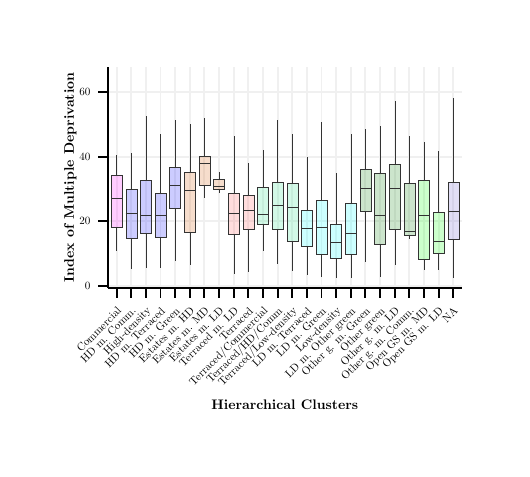
\begin{tikzpicture}[x=1pt,y=1pt]
\definecolor{fillColor}{RGB}{255,255,255}
\path[use as bounding box,fill=fillColor,fill opacity=0.00] (0,0) rectangle (171.17,152.15);
\begin{scope}
\path[clip] (  0.00,  0.00) rectangle (171.17,152.15);
\definecolor{fillColor}{RGB}{255,255,255}

\path[fill=fillColor] (  0.00,  0.00) rectangle (171.17,152.15);
\end{scope}
\begin{scope}
\path[clip] ( 28.95, 58.04) rectangle (156.94,137.92);
\definecolor{fillColor}{RGB}{255,255,255}

\path[fill=fillColor] ( 28.95, 58.04) rectangle (156.94,137.92);
\definecolor{drawColor}{gray}{0.94}

\path[draw=drawColor,line width= 0.7pt,line join=round] ( 28.95, 58.96) --
	(156.94, 58.96);

\path[draw=drawColor,line width= 0.7pt,line join=round] ( 28.95, 82.25) --
	(156.94, 82.25);

\path[draw=drawColor,line width= 0.7pt,line join=round] ( 28.95,105.55) --
	(156.94,105.55);

\path[draw=drawColor,line width= 0.7pt,line join=round] ( 28.95,128.84) --
	(156.94,128.84);

\path[draw=drawColor,line width= 0.7pt,line join=round] ( 32.12, 58.04) --
	( 32.12,137.92);

\path[draw=drawColor,line width= 0.7pt,line join=round] ( 37.41, 58.04) --
	( 37.41,137.92);

\path[draw=drawColor,line width= 0.7pt,line join=round] ( 42.70, 58.04) --
	( 42.70,137.92);

\path[draw=drawColor,line width= 0.7pt,line join=round] ( 47.99, 58.04) --
	( 47.99,137.92);

\path[draw=drawColor,line width= 0.7pt,line join=round] ( 53.28, 58.04) --
	( 53.28,137.92);

\path[draw=drawColor,line width= 0.7pt,line join=round] ( 58.57, 58.04) --
	( 58.57,137.92);

\path[draw=drawColor,line width= 0.7pt,line join=round] ( 63.85, 58.04) --
	( 63.85,137.92);

\path[draw=drawColor,line width= 0.7pt,line join=round] ( 69.14, 58.04) --
	( 69.14,137.92);

\path[draw=drawColor,line width= 0.7pt,line join=round] ( 74.43, 58.04) --
	( 74.43,137.92);

\path[draw=drawColor,line width= 0.7pt,line join=round] ( 79.72, 58.04) --
	( 79.72,137.92);

\path[draw=drawColor,line width= 0.7pt,line join=round] ( 85.01, 58.04) --
	( 85.01,137.92);

\path[draw=drawColor,line width= 0.7pt,line join=round] ( 90.30, 58.04) --
	( 90.30,137.92);

\path[draw=drawColor,line width= 0.7pt,line join=round] ( 95.59, 58.04) --
	( 95.59,137.92);

\path[draw=drawColor,line width= 0.7pt,line join=round] (100.88, 58.04) --
	(100.88,137.92);

\path[draw=drawColor,line width= 0.7pt,line join=round] (106.17, 58.04) --
	(106.17,137.92);

\path[draw=drawColor,line width= 0.7pt,line join=round] (111.45, 58.04) --
	(111.45,137.92);

\path[draw=drawColor,line width= 0.7pt,line join=round] (116.74, 58.04) --
	(116.74,137.92);

\path[draw=drawColor,line width= 0.7pt,line join=round] (122.03, 58.04) --
	(122.03,137.92);

\path[draw=drawColor,line width= 0.7pt,line join=round] (127.32, 58.04) --
	(127.32,137.92);

\path[draw=drawColor,line width= 0.7pt,line join=round] (132.61, 58.04) --
	(132.61,137.92);

\path[draw=drawColor,line width= 0.7pt,line join=round] (137.90, 58.04) --
	(137.90,137.92);

\path[draw=drawColor,line width= 0.7pt,line join=round] (143.19, 58.04) --
	(143.19,137.92);

\path[draw=drawColor,line width= 0.7pt,line join=round] (148.48, 58.04) --
	(148.48,137.92);

\path[draw=drawColor,line width= 0.7pt,line join=round] (153.77, 58.04) --
	(153.77,137.92);
\definecolor{drawColor}{gray}{0.20}

\path[draw=drawColor,line width= 0.1pt,line join=round] ( 37.41, 93.83) -- ( 37.41,106.70);

\path[draw=drawColor,line width= 0.1pt,line join=round] ( 37.41, 75.96) -- ( 37.41, 64.95);
\definecolor{fillColor}{RGB}{0,0,255}

\path[draw=drawColor,line width= 0.1pt,fill=fillColor,fill opacity=0.20] ( 35.43, 93.83) --
	( 35.43, 75.96) --
	( 39.39, 75.96) --
	( 39.39, 93.83) --
	( 35.43, 93.83) --
	cycle;

\path[draw=drawColor,line width= 0.1pt] ( 35.43, 85.16) -- ( 39.39, 85.16);

\path[draw=drawColor,line width= 0.1pt,line join=round] ( 42.70, 97.11) -- ( 42.70,120.18);

\path[draw=drawColor,line width= 0.1pt,line join=round] ( 42.70, 77.78) -- ( 42.70, 65.22);

\path[draw=drawColor,line width= 0.1pt,fill=fillColor,fill opacity=0.20] ( 40.72, 97.11) --
	( 40.72, 77.78) --
	( 44.68, 77.78) --
	( 44.68, 97.11) --
	( 40.72, 97.11) --
	cycle;

\path[draw=drawColor,line width= 0.1pt] ( 40.72, 84.25) -- ( 44.68, 84.25);

\path[draw=drawColor,line width= 0.1pt,line join=round] ( 32.12, 98.85) -- ( 32.12,106.18);

\path[draw=drawColor,line width= 0.1pt,line join=round] ( 32.12, 80.15) -- ( 32.12, 71.61);
\definecolor{fillColor}{RGB}{255,0,255}

\path[draw=drawColor,line width= 0.1pt,fill=fillColor,fill opacity=0.20] ( 30.14, 98.85) --
	( 30.14, 80.15) --
	( 34.10, 80.15) --
	( 34.10, 98.85) --
	( 30.14, 98.85) --
	cycle;

\path[draw=drawColor,line width= 0.1pt] ( 30.14, 90.59) -- ( 34.10, 90.59);

\path[draw=drawColor,line width= 0.1pt,line join=round] (100.88, 86.12) -- (100.88,105.53);

\path[draw=drawColor,line width= 0.1pt,line join=round] (100.88, 73.09) -- (100.88, 62.82);
\definecolor{fillColor}{RGB}{0,255,255}

\path[draw=drawColor,line width= 0.1pt,fill=fillColor,fill opacity=0.20] ( 98.89, 86.12) --
	( 98.89, 73.09) --
	(102.86, 73.09) --
	(102.86, 86.12) --
	( 98.89, 86.12) --
	cycle;

\path[draw=drawColor,line width= 0.1pt] ( 98.89, 79.65) -- (102.86, 79.65);

\path[draw=drawColor,line width= 0.1pt,line join=round] (106.17, 89.96) -- (106.17,118.02);

\path[draw=drawColor,line width= 0.1pt,line join=round] (106.17, 70.38) -- (106.17, 61.95);

\path[draw=drawColor,line width= 0.1pt,fill=fillColor,fill opacity=0.20] (104.18, 89.96) --
	(104.18, 70.38) --
	(108.15, 70.38) --
	(108.15, 89.96) --
	(104.18, 89.96) --
	cycle;

\path[draw=drawColor,line width= 0.1pt] (104.18, 80.16) -- (108.15, 80.16);

\path[draw=drawColor,line width= 0.1pt,line join=round] (132.61,102.72) -- (132.61,125.63);

\path[draw=drawColor,line width= 0.1pt,line join=round] (132.61, 79.21) -- (132.61, 66.25);
\definecolor{fillColor}{RGB}{0,128,0}

\path[draw=drawColor,line width= 0.1pt,fill=fillColor,fill opacity=0.20] (130.63,102.72) --
	(130.63, 79.21) --
	(134.59, 79.21) --
	(134.59,102.72) --
	(130.63,102.72) --
	cycle;

\path[draw=drawColor,line width= 0.1pt] (130.63, 94.15) -- (134.59, 94.15);

\path[draw=drawColor,line width= 0.1pt,line join=round] ( 74.43, 92.26) -- ( 74.43,113.05);

\path[draw=drawColor,line width= 0.1pt,line join=round] ( 74.43, 77.65) -- ( 74.43, 63.12);
\definecolor{fillColor}{RGB}{255,85,85}

\path[draw=drawColor,line width= 0.1pt,fill=fillColor,fill opacity=0.20] ( 72.45, 92.26) --
	( 72.45, 77.65) --
	( 76.42, 77.65) --
	( 76.42, 92.26) --
	( 72.45, 92.26) --
	cycle;

\path[draw=drawColor,line width= 0.1pt] ( 72.45, 85.23) -- ( 76.42, 85.23);

\path[draw=drawColor,line width= 0.1pt,line join=round] ( 53.28,101.81) -- ( 53.28,118.83);

\path[draw=drawColor,line width= 0.1pt,line join=round] ( 53.28, 86.83) -- ( 53.28, 67.96);
\definecolor{fillColor}{RGB}{0,0,255}

\path[draw=drawColor,line width= 0.1pt,fill=fillColor,fill opacity=0.20] ( 51.29,101.81) --
	( 51.29, 86.83) --
	( 55.26, 86.83) --
	( 55.26,101.81) --
	( 51.29,101.81) --
	cycle;

\path[draw=drawColor,line width= 0.1pt] ( 51.29, 95.23) -- ( 55.26, 95.23);

\path[draw=drawColor,line width= 0.1pt,line join=round] ( 79.72, 91.53) -- ( 79.72,103.08);

\path[draw=drawColor,line width= 0.1pt,line join=round] ( 79.72, 79.39) -- ( 79.72, 64.04);
\definecolor{fillColor}{RGB}{255,85,85}

\path[draw=drawColor,line width= 0.1pt,fill=fillColor,fill opacity=0.20] ( 77.74, 91.53) --
	( 77.74, 79.39) --
	( 81.70, 79.39) --
	( 81.70, 91.53) --
	( 77.74, 91.53) --
	cycle;

\path[draw=drawColor,line width= 0.1pt] ( 77.74, 86.15) -- ( 81.70, 86.15);

\path[draw=drawColor,line width= 0.1pt,line join=round] ( 47.99, 92.49) -- ( 47.99,113.77);

\path[draw=drawColor,line width= 0.1pt,line join=round] ( 47.99, 76.41) -- ( 47.99, 65.30);
\definecolor{fillColor}{RGB}{0,0,255}

\path[draw=drawColor,line width= 0.1pt,fill=fillColor,fill opacity=0.20] ( 46.00, 92.49) --
	( 46.00, 76.41) --
	( 49.97, 76.41) --
	( 49.97, 92.49) --
	( 46.00, 92.49) --
	cycle;

\path[draw=drawColor,line width= 0.1pt] ( 46.00, 84.57) -- ( 49.97, 84.57);

\path[draw=drawColor,line width= 0.1pt,line join=round] (116.74, 88.64) -- (116.74,113.57);

\path[draw=drawColor,line width= 0.1pt,line join=round] (116.74, 70.35) -- (116.74, 61.68);
\definecolor{fillColor}{RGB}{0,255,255}

\path[draw=drawColor,line width= 0.1pt,fill=fillColor,fill opacity=0.20] (114.76, 88.64) --
	(114.76, 70.35) --
	(118.73, 70.35) --
	(118.73, 88.64) --
	(114.76, 88.64) --
	cycle;

\path[draw=drawColor,line width= 0.1pt] (114.76, 77.87) -- (118.73, 77.87);

\path[draw=drawColor,line width= 0.1pt,line join=round] (111.45, 81.17) -- (111.45, 99.67);

\path[draw=drawColor,line width= 0.1pt,line join=round] (111.45, 68.76) -- (111.45, 61.67);

\path[draw=drawColor,line width= 0.1pt,fill=fillColor,fill opacity=0.20] (109.47, 81.17) --
	(109.47, 68.76) --
	(113.44, 68.76) --
	(113.44, 81.17) --
	(109.47, 81.17) --
	cycle;

\path[draw=drawColor,line width= 0.1pt] (109.47, 74.68) -- (113.44, 74.68);

\path[draw=drawColor,line width= 0.1pt,line join=round] (127.32, 99.67) -- (127.32,116.72);

\path[draw=drawColor,line width= 0.1pt,line join=round] (127.32, 73.90) -- (127.32, 62.16);
\definecolor{fillColor}{RGB}{0,128,0}

\path[draw=drawColor,line width= 0.1pt,fill=fillColor,fill opacity=0.20] (125.34, 99.67) --
	(125.34, 73.90) --
	(129.30, 73.90) --
	(129.30, 99.67) --
	(125.34, 99.67) --
	cycle;

\path[draw=drawColor,line width= 0.1pt] (125.34, 84.45) -- (129.30, 84.45);

\path[draw=drawColor,line width= 0.1pt,line join=round] (122.03,101.13) -- (122.03,115.54);

\path[draw=drawColor,line width= 0.1pt,line join=round] (122.03, 85.81) -- (122.03, 67.49);

\path[draw=drawColor,line width= 0.1pt,fill=fillColor,fill opacity=0.20] (120.05,101.13) --
	(120.05, 85.81) --
	(124.02, 85.81) --
	(124.02,101.13) --
	(120.05,101.13) --
	cycle;

\path[draw=drawColor,line width= 0.1pt] (120.05, 94.34) -- (124.02, 94.34);

\path[draw=drawColor,line width= 0.1pt,line join=round] ( 95.59, 96.08) -- ( 95.59,113.61);

\path[draw=drawColor,line width= 0.1pt,line join=round] ( 95.59, 75.18) -- ( 95.59, 64.18);
\definecolor{fillColor}{RGB}{37,229,137}

\path[draw=drawColor,line width= 0.1pt,fill=fillColor,fill opacity=0.20] ( 93.60, 96.08) --
	( 93.60, 75.18) --
	( 97.57, 75.18) --
	( 97.57, 96.08) --
	( 93.60, 96.08) --
	cycle;

\path[draw=drawColor,line width= 0.1pt] ( 93.60, 87.13) -- ( 97.57, 87.13);

\path[draw=drawColor,line width= 0.1pt,line join=round] (148.48, 85.34) -- (148.48,107.43);

\path[draw=drawColor,line width= 0.1pt,line join=round] (148.48, 70.54) -- (148.48, 64.58);
\definecolor{fillColor}{RGB}{0,255,0}

\path[draw=drawColor,line width= 0.1pt,fill=fillColor,fill opacity=0.20] (146.49, 85.34) --
	(146.49, 70.54) --
	(150.46, 70.54) --
	(150.46, 85.34) --
	(146.49, 85.34) --
	cycle;

\path[draw=drawColor,line width= 0.1pt] (146.49, 75.18) -- (150.46, 75.18);

\path[draw=drawColor,line width= 0.1pt,line join=round] ( 90.30, 96.50) -- ( 90.30,118.85);

\path[draw=drawColor,line width= 0.1pt,line join=round] ( 90.30, 79.45) -- ( 90.30, 66.77);
\definecolor{fillColor}{RGB}{37,229,137}

\path[draw=drawColor,line width= 0.1pt,fill=fillColor,fill opacity=0.20] ( 88.32, 96.50) --
	( 88.32, 79.45) --
	( 92.28, 79.45) --
	( 92.28, 96.50) --
	( 88.32, 96.50) --
	cycle;

\path[draw=drawColor,line width= 0.1pt] ( 88.32, 87.92) -- ( 92.28, 87.92);

\path[draw=drawColor,line width= 0.1pt,line join=round] ( 58.57,100.07) -- ( 58.57,117.31);

\path[draw=drawColor,line width= 0.1pt,line join=round] ( 58.57, 78.29) -- ( 58.57, 66.40);
\definecolor{fillColor}{RGB}{212,85,0}

\path[draw=drawColor,line width= 0.1pt,fill=fillColor,fill opacity=0.20] ( 56.58,100.07) --
	( 56.58, 78.29) --
	( 60.55, 78.29) --
	( 60.55,100.07) --
	( 56.58,100.07) --
	cycle;

\path[draw=drawColor,line width= 0.1pt] ( 56.58, 93.50) -- ( 60.55, 93.50);

\path[draw=drawColor,line width= 0.1pt,line join=round] (143.19, 97.18) -- (143.19,110.98);

\path[draw=drawColor,line width= 0.1pt,line join=round] (143.19, 68.44) -- (143.19, 64.43);
\definecolor{fillColor}{RGB}{0,255,0}

\path[draw=drawColor,line width= 0.1pt,fill=fillColor,fill opacity=0.20] (141.20, 97.18) --
	(141.20, 68.44) --
	(145.17, 68.44) --
	(145.17, 97.18) --
	(141.20, 97.18) --
	cycle;

\path[draw=drawColor,line width= 0.1pt] (141.20, 84.27) -- (145.17, 84.27);

\path[draw=drawColor,line width= 0.1pt,line join=round] ( 85.01, 94.38) -- ( 85.01,108.01);

\path[draw=drawColor,line width= 0.1pt,line join=round] ( 85.01, 81.32) -- ( 85.01, 71.37);
\definecolor{fillColor}{RGB}{37,229,137}

\path[draw=drawColor,line width= 0.1pt,fill=fillColor,fill opacity=0.20] ( 83.03, 94.38) --
	( 83.03, 81.32) --
	( 86.99, 81.32) --
	( 86.99, 94.38) --
	( 83.03, 94.38) --
	cycle;

\path[draw=drawColor,line width= 0.1pt] ( 83.03, 84.69) -- ( 86.99, 84.69);

\path[draw=drawColor,line width= 0.1pt,line join=round] ( 63.85,105.71) -- ( 63.85,119.48);

\path[draw=drawColor,line width= 0.1pt,line join=round] ( 63.85, 95.28) -- ( 63.85, 90.61);
\definecolor{fillColor}{RGB}{212,85,0}

\path[draw=drawColor,line width= 0.1pt,fill=fillColor,fill opacity=0.20] ( 61.87,105.71) --
	( 61.87, 95.28) --
	( 65.84, 95.28) --
	( 65.84,105.71) --
	( 61.87,105.71) --
	cycle;

\path[draw=drawColor,line width= 0.1pt] ( 61.87,103.31) -- ( 65.84,103.31);

\path[draw=drawColor,line width= 0.1pt,line join=round] ( 69.14, 97.39) -- ( 69.14,100.03);

\path[draw=drawColor,line width= 0.1pt,line join=round] ( 69.14, 93.66) -- ( 69.14, 92.36);

\path[draw=drawColor,line width= 0.1pt,fill=fillColor,fill opacity=0.20] ( 67.16, 97.39) --
	( 67.16, 93.66) --
	( 71.13, 93.66) --
	( 71.13, 97.39) --
	( 67.16, 97.39) --
	cycle;

\path[draw=drawColor,line width= 0.1pt] ( 67.16, 95.01) -- ( 71.13, 95.01);

\path[draw=drawColor,line width= 0.1pt,line join=round] (137.90, 95.89) -- (137.90,112.99);

\path[draw=drawColor,line width= 0.1pt,line join=round] (137.90, 77.24) -- (137.90, 75.70);
\definecolor{fillColor}{RGB}{0,128,0}

\path[draw=drawColor,line width= 0.1pt,fill=fillColor,fill opacity=0.20] (135.92, 95.89) --
	(135.92, 77.24) --
	(139.88, 77.24) --
	(139.88, 95.89) --
	(135.92, 95.89) --
	cycle;

\path[draw=drawColor,line width= 0.1pt] (135.92, 78.78) -- (139.88, 78.78);

\path[draw=drawColor,line width= 0.1pt,line join=round] (153.77, 96.40) -- (153.77,126.71);

\path[draw=drawColor,line width= 0.1pt,line join=round] (153.77, 75.64) -- (153.77, 61.82);
\definecolor{fillColor}{RGB}{106,90,205}

\path[draw=drawColor,line width= 0.1pt,fill=fillColor,fill opacity=0.20] (151.78, 96.40) --
	(151.78, 75.64) --
	(155.75, 75.64) --
	(155.75, 96.40) --
	(151.78, 96.40) --
	cycle;

\path[draw=drawColor,line width= 0.1pt] (151.78, 85.81) -- (155.75, 85.81);

\path[] ( 28.95, 58.04) rectangle (156.94,137.92);
\end{scope}
\begin{scope}
\path[clip] (  0.00,  0.00) rectangle (171.17,152.15);
\definecolor{drawColor}{RGB}{0,0,0}

\path[draw=drawColor,line width= 0.7pt,line join=round] ( 28.95, 58.04) --
	( 28.95,137.92);
\end{scope}
\begin{scope}
\path[clip] (  0.00,  0.00) rectangle (171.17,152.15);
\definecolor{drawColor}{RGB}{0,0,0}

\node[text=drawColor,anchor=base east,inner sep=0pt, outer sep=0pt, scale=  0.40] at ( 22.65, 57.58) {0};

\node[text=drawColor,anchor=base east,inner sep=0pt, outer sep=0pt, scale=  0.40] at ( 22.65, 80.88) {20};

\node[text=drawColor,anchor=base east,inner sep=0pt, outer sep=0pt, scale=  0.40] at ( 22.65,104.17) {40};

\node[text=drawColor,anchor=base east,inner sep=0pt, outer sep=0pt, scale=  0.40] at ( 22.65,127.47) {60};
\end{scope}
\begin{scope}
\path[clip] (  0.00,  0.00) rectangle (171.17,152.15);
\definecolor{drawColor}{RGB}{0,0,0}

\path[draw=drawColor,line width= 0.7pt,line join=round] ( 25.45, 58.96) --
	( 28.95, 58.96);

\path[draw=drawColor,line width= 0.7pt,line join=round] ( 25.45, 82.25) --
	( 28.95, 82.25);

\path[draw=drawColor,line width= 0.7pt,line join=round] ( 25.45,105.55) --
	( 28.95,105.55);

\path[draw=drawColor,line width= 0.7pt,line join=round] ( 25.45,128.84) --
	( 28.95,128.84);
\end{scope}
\begin{scope}
\path[clip] (  0.00,  0.00) rectangle (171.17,152.15);
\definecolor{drawColor}{RGB}{0,0,0}

\path[draw=drawColor,line width= 0.7pt,line join=round] ( 28.95, 58.04) --
	(156.94, 58.04);
\end{scope}
\begin{scope}
\path[clip] (  0.00,  0.00) rectangle (171.17,152.15);
\definecolor{drawColor}{RGB}{0,0,0}

\path[draw=drawColor,line width= 0.7pt,line join=round] ( 32.12, 54.54) --
	( 32.12, 58.04);

\path[draw=drawColor,line width= 0.7pt,line join=round] ( 37.41, 54.54) --
	( 37.41, 58.04);

\path[draw=drawColor,line width= 0.7pt,line join=round] ( 42.70, 54.54) --
	( 42.70, 58.04);

\path[draw=drawColor,line width= 0.7pt,line join=round] ( 47.99, 54.54) --
	( 47.99, 58.04);

\path[draw=drawColor,line width= 0.7pt,line join=round] ( 53.28, 54.54) --
	( 53.28, 58.04);

\path[draw=drawColor,line width= 0.7pt,line join=round] ( 58.57, 54.54) --
	( 58.57, 58.04);

\path[draw=drawColor,line width= 0.7pt,line join=round] ( 63.85, 54.54) --
	( 63.85, 58.04);

\path[draw=drawColor,line width= 0.7pt,line join=round] ( 69.14, 54.54) --
	( 69.14, 58.04);

\path[draw=drawColor,line width= 0.7pt,line join=round] ( 74.43, 54.54) --
	( 74.43, 58.04);

\path[draw=drawColor,line width= 0.7pt,line join=round] ( 79.72, 54.54) --
	( 79.72, 58.04);

\path[draw=drawColor,line width= 0.7pt,line join=round] ( 85.01, 54.54) --
	( 85.01, 58.04);

\path[draw=drawColor,line width= 0.7pt,line join=round] ( 90.30, 54.54) --
	( 90.30, 58.04);

\path[draw=drawColor,line width= 0.7pt,line join=round] ( 95.59, 54.54) --
	( 95.59, 58.04);

\path[draw=drawColor,line width= 0.7pt,line join=round] (100.88, 54.54) --
	(100.88, 58.04);

\path[draw=drawColor,line width= 0.7pt,line join=round] (106.17, 54.54) --
	(106.17, 58.04);

\path[draw=drawColor,line width= 0.7pt,line join=round] (111.45, 54.54) --
	(111.45, 58.04);

\path[draw=drawColor,line width= 0.7pt,line join=round] (116.74, 54.54) --
	(116.74, 58.04);

\path[draw=drawColor,line width= 0.7pt,line join=round] (122.03, 54.54) --
	(122.03, 58.04);

\path[draw=drawColor,line width= 0.7pt,line join=round] (127.32, 54.54) --
	(127.32, 58.04);

\path[draw=drawColor,line width= 0.7pt,line join=round] (132.61, 54.54) --
	(132.61, 58.04);

\path[draw=drawColor,line width= 0.7pt,line join=round] (137.90, 54.54) --
	(137.90, 58.04);

\path[draw=drawColor,line width= 0.7pt,line join=round] (143.19, 54.54) --
	(143.19, 58.04);

\path[draw=drawColor,line width= 0.7pt,line join=round] (148.48, 54.54) --
	(148.48, 58.04);

\path[draw=drawColor,line width= 0.7pt,line join=round] (153.77, 54.54) --
	(153.77, 58.04);
\end{scope}
\begin{scope}
\path[clip] (  0.00,  0.00) rectangle (171.17,152.15);
\definecolor{drawColor}{RGB}{0,0,0}

\node[text=drawColor,rotate= 45.00,anchor=base east,inner sep=0pt, outer sep=0pt, scale=  0.40] at ( 34.05, 49.51) {Commercial};

\node[text=drawColor,rotate= 45.00,anchor=base east,inner sep=0pt, outer sep=0pt, scale=  0.40] at ( 39.34, 49.51) {HD m. Comm.};

\node[text=drawColor,rotate= 45.00,anchor=base east,inner sep=0pt, outer sep=0pt, scale=  0.40] at ( 44.63, 49.51) {High-density};

\node[text=drawColor,rotate= 45.00,anchor=base east,inner sep=0pt, outer sep=0pt, scale=  0.40] at ( 49.92, 49.51) {HD m. Terraced};

\node[text=drawColor,rotate= 45.00,anchor=base east,inner sep=0pt, outer sep=0pt, scale=  0.40] at ( 55.21, 49.51) {HD m. Green};

\node[text=drawColor,rotate= 45.00,anchor=base east,inner sep=0pt, outer sep=0pt, scale=  0.40] at ( 60.49, 49.51) {Estates m. HD};

\node[text=drawColor,rotate= 45.00,anchor=base east,inner sep=0pt, outer sep=0pt, scale=  0.40] at ( 65.78, 49.51) {Estates m. MD};

\node[text=drawColor,rotate= 45.00,anchor=base east,inner sep=0pt, outer sep=0pt, scale=  0.40] at ( 71.07, 49.51) {Estates m. LD};

\node[text=drawColor,rotate= 45.00,anchor=base east,inner sep=0pt, outer sep=0pt, scale=  0.40] at ( 76.36, 49.51) {Terraced m. LD};

\node[text=drawColor,rotate= 45.00,anchor=base east,inner sep=0pt, outer sep=0pt, scale=  0.40] at ( 81.65, 49.51) {Terraced};

\node[text=drawColor,rotate= 45.00,anchor=base east,inner sep=0pt, outer sep=0pt, scale=  0.40] at ( 86.94, 49.51) {Terraced/Commercial};

\node[text=drawColor,rotate= 45.00,anchor=base east,inner sep=0pt, outer sep=0pt, scale=  0.40] at ( 92.23, 49.51) {Terraced/HD/Comm};

\node[text=drawColor,rotate= 45.00,anchor=base east,inner sep=0pt, outer sep=0pt, scale=  0.40] at ( 97.52, 49.51) {Terraced/Low-density};

\node[text=drawColor,rotate= 45.00,anchor=base east,inner sep=0pt, outer sep=0pt, scale=  0.40] at (102.81, 49.51) {LD m. Terraced};

\node[text=drawColor,rotate= 45.00,anchor=base east,inner sep=0pt, outer sep=0pt, scale=  0.40] at (108.09, 49.51) {LD m. Green};

\node[text=drawColor,rotate= 45.00,anchor=base east,inner sep=0pt, outer sep=0pt, scale=  0.40] at (113.38, 49.51) {Low-density};

\node[text=drawColor,rotate= 45.00,anchor=base east,inner sep=0pt, outer sep=0pt, scale=  0.40] at (118.67, 49.51) {LD m. Other green};

\node[text=drawColor,rotate= 45.00,anchor=base east,inner sep=0pt, outer sep=0pt, scale=  0.40] at (123.96, 49.51) {Other g. m. Green};

\node[text=drawColor,rotate= 45.00,anchor=base east,inner sep=0pt, outer sep=0pt, scale=  0.40] at (129.25, 49.51) {Other green};

\node[text=drawColor,rotate= 45.00,anchor=base east,inner sep=0pt, outer sep=0pt, scale=  0.40] at (134.54, 49.51) {Other g. m. LD};

\node[text=drawColor,rotate= 45.00,anchor=base east,inner sep=0pt, outer sep=0pt, scale=  0.40] at (139.83, 49.51) {Other g. m. Comm.};

\node[text=drawColor,rotate= 45.00,anchor=base east,inner sep=0pt, outer sep=0pt, scale=  0.40] at (145.12, 49.51) {Open GS m. MD};

\node[text=drawColor,rotate= 45.00,anchor=base east,inner sep=0pt, outer sep=0pt, scale=  0.40] at (150.41, 49.51) {Open GS m. LD};

\node[text=drawColor,rotate= 45.00,anchor=base east,inner sep=0pt, outer sep=0pt, scale=  0.40] at (155.69, 49.51) {NA};
\end{scope}
\begin{scope}
\path[clip] (  0.00,  0.00) rectangle (171.17,152.15);
\definecolor{drawColor}{RGB}{0,0,0}

\node[text=drawColor,anchor=base,inner sep=0pt, outer sep=0pt, scale=  0.50] at ( 92.94, 14.03) {\bfseries Hierarchical Clusters};
\end{scope}
\begin{scope}
\path[clip] (  0.00,  0.00) rectangle (171.17,152.15);
\definecolor{drawColor}{RGB}{0,0,0}

\node[text=drawColor,rotate= 90.00,anchor=base,inner sep=0pt, outer sep=0pt, scale=  0.50] at ( 16.70, 97.98) {\bfseries Index of Multiple Deprivation};
\end{scope}
\end{tikzpicture}
